\sectionquestion{Regression and Optimization}

\begin{parts}

\part Suppose you have a regression dataset with one input feature, $x$, and one output value $y$. You wish to evaluate various regression techniques.

\begin{subparts}
    \subpart[2] \textbf{Drawing:} Draw the function that a linear regression model would learn on the dataset below.

    \begin{center}
    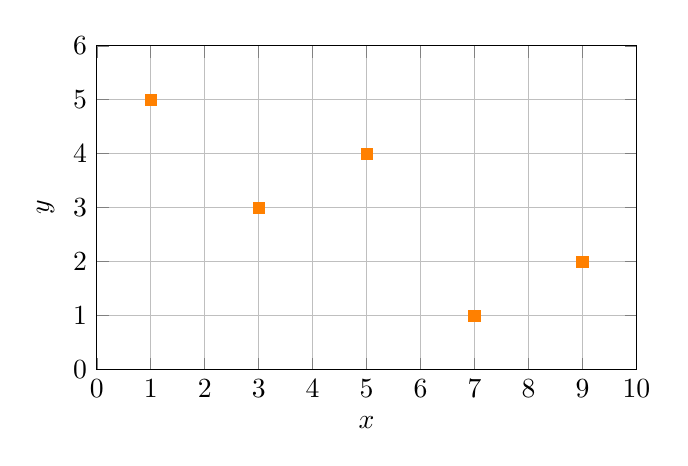
\begin{tikzpicture}
    \begin{axis}[
        scale=1.0, axis equal image,
        xmin=0, xmax=10, xtick={0,...,10},
        ymin=0, ymax=6, ytick={0,...,6},
        samples=50, grid=major, xlabel=$x$, ylabel=$y$]
        \addplot [
            scatter,
            only marks,
            point meta=explicit symbolic,
            scatter/classes={
                a={mark=square*,orange},
                b={mark=triangle*,red}
            },
            nodes near coords*={},
            visualization depends on={\thisrow{myvalue} \as \myvalue},
        ] table [meta=label] {
            x y label myvalue
            1 5 a 1
            3 3 a 1
            5 4 a 1
            7 1 a 1
            9 2 a 1
        };
    \end{axis}
    \end{tikzpicture}
    \end{center}
    \begin{soln} Any straight line that roughly passes through the points should get full credit. \end{soln}
    \begin{qauthor} Matt (Solution by Henry) \end{qauthor}

    \subpart[2] \textbf{Drawing:} Draw the function that a $k$-nearest neighbor regression model with $k=1$ would learn on the dataset below.

    \begin{center}
    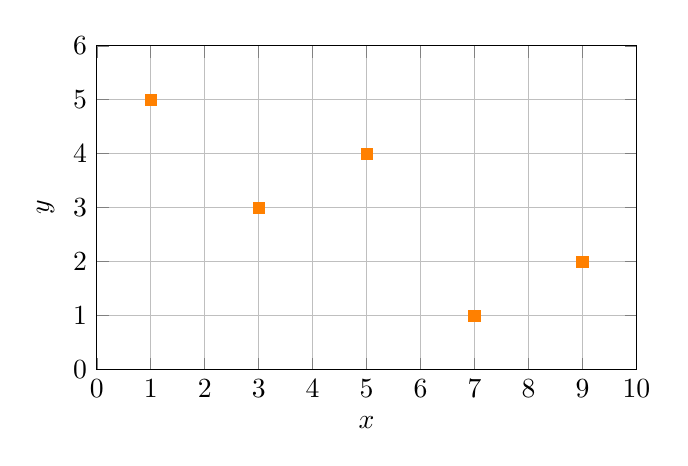
\begin{tikzpicture}
    \begin{axis}[
        scale=1.0, axis equal image,
        xmin=0, xmax=10, xtick={0,...,10},
        ymin=0, ymax=6, ytick={0,...,6},
        samples=50, grid=major, xlabel=$x$, ylabel=$y$]
        \addplot [
            scatter,
            only marks,
            point meta=explicit symbolic,
            scatter/classes={
                a={mark=square*,orange},
                b={mark=triangle*,red}
            },
            nodes near coords*={},
            visualization depends on={\thisrow{myvalue} \as \myvalue},
        ] table [meta=label] {
            x y label myvalue
            1 5 a 1
            3 3 a 1
            5 4 a 1
            7 1 a 1
            9 2 a 1
        };
    \end{axis}
    \end{tikzpicture}
    \end{center}
    \begin{soln} Piecewise linear with all components parallel to the x-axis, passing through the points, i.e., line segment from $x\in [0,2]$ at $y=5$, then $x\in [2,4]$ at $y=3$ etc... \end{soln}
    \begin{qauthor} Matt (Solution by Henry) \end{qauthor}
    
    \subpart[2] \textbf{Drawing:} Draw the function that a decision tree regression model with features of the form $x < c$ would learn on the dataset below.

    \begin{center}
    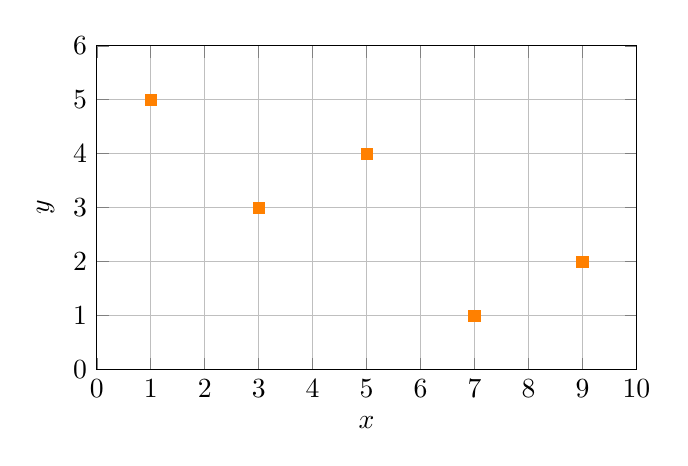
\begin{tikzpicture}
    \begin{axis}[
        scale=1.0, axis equal image,
        xmin=0, xmax=10, xtick={0,...,10},
        ymin=0, ymax=6, ytick={0,...,6},
        samples=50, grid=major, xlabel=$x$, ylabel=$y$]
        \addplot [
            scatter,
            only marks,
            point meta=explicit symbolic,
            scatter/classes={
                a={mark=square*,orange},
                b={mark=triangle*,red}
            },
            nodes near coords*={},
            visualization depends on={\thisrow{myvalue} \as \myvalue},
        ] table [meta=label] {
            x y label myvalue
            1 5 a 1
            3 3 a 1
            5 4 a 1
            7 1 a 1
            9 2 a 1
        };
    \end{axis}
    \end{tikzpicture}
    \end{center}
    \begin{soln} Very similar to part (b) except the line segments to do not need to end exactly at the midpoints between the orange squares; should still be piecewise linear with components parallel to the x-axis. \end{soln}
    \begin{qauthor} Matt (Solution by Henry) \end{qauthor}
\end{subparts}
    
\part We wish to learn a linear regression model on data $\Dc = \{ (\xv^{(i)}, y^{(i)}) \}_{i=1}^N$ For this question, define the pointwise exponential squared error as
\[
    J^{(i)}\Big(\thetav\Big)=\textrm{exp}\bigg(\frac{1}{2}\Big(y^{(i)} - \thetav^T\xv^{(i)}\Big)^2\bigg)
\]
Suppose we are interested in minimizing the \emph{geometric} mean of the exponential squared errors over our training data. Recall that the geometric mean of a set of values \\ $\{x^{(1)}, \ldots, x^{(n)}\}$ is the $n^{\textrm{th}}$ root of their product. Thus, our objective in this setting is
\[
    J\Big(\thetav\Big)=\bigg(\prod_{i=1}^N J^{(i)}(\thetav)\bigg)^{\frac{1}{N}}
\]

\begin{subparts}
    \subpart[2] \textbf{Math:} What is the partial derivative of $J^{(i)}\Big(\thetav\Big)$ with respect to the $k^{\textrm{th}}$ parameter, $\theta_k$?
    \begin{tcolorbox}[fit,height=3cm, width=15cm, blank, borderline={1pt}{-2pt}]
        %solution
    \end{tcolorbox}
    \begin{soln}
        \begin{align}
            \frac{\partial J^{(i)}}{\partial \theta_j} &= \frac{\partial}{\partial \theta_j}\Bigg(\textrm{exp}\bigg(\frac{1}{2}\Big(y^{(i)} - \vec{\theta}^T\vec{x}^{(i)}\Big)^2\bigg)\Bigg) \nonumber \\ 
            &= \textrm{exp}\bigg(\frac{1}{2}\Big(y^{(i)} - \vec{\theta}^T\vec{x}^{(i)}\Big)^2\bigg)\frac{\partial}{\partial \theta_j}\frac{1}{2}\Big(y^{(i)} - \vec{\theta}^T\vec{x}^{(i)}\Big)^2 \nonumber \\
            &= \textrm{exp}\bigg(\frac{1}{2}\Big(y^{(i)} - \vec{\theta}^T\vec{x}^{(i)}\Big)^2\bigg)\Big(y^{(i)} - \vec{\theta}^T\vec{x}^{(i)}\Big)\Big(-x^{(i)}_j\Big) \nonumber
        \end{align}
    \end{soln}
    \begin{qauthor}
       Henry
    \end{qauthor}
    
    \subpart[2] \textbf{Math:} What is the gradient of $J^{(i)}\Big(\thetav\Big)$ with respect to the vector $\thetav$?
    \begin{tcolorbox}[fit,height=3cm, width=15cm, blank, borderline={1pt}{-2pt}]
        %solution
    \end{tcolorbox}
    \begin{soln}
        \begin{align}
            \frac{\partial J^{(i)}}{\partial \vec{\theta}} &= \frac{\partial}{\partial \vec{\theta}}\Bigg(\textrm{exp}\bigg(\frac{1}{2}\Big(y^{(i)} - \vec{\theta}^T\vec{x}^{(i)}\Big)^2\bigg)\Bigg) \nonumber \\ 
            &= \textrm{exp}\bigg(\frac{1}{2}\Big(y^{(i)} - \vec{\theta}^T\vec{x}^{(i)}\Big)^2\bigg)\frac{\partial}{\partial \vec{\theta}}\frac{1}{2}\Big(y^{(i)} - \vec{\theta}^T\vec{x}^{(i)}\Big)^2 \nonumber \\
            &= \textrm{exp}\bigg(\frac{1}{2}\Big(y^{(i)} - \vec{\theta}^T\vec{x}^{(i)}\Big)^2\bigg)\Big(y^{(i)} - \vec{\theta}^T\vec{x}^{(i)}\Big)\Big(-\vec{x}^{(i)}\Big) \nonumber
        \end{align}
    \end{soln}
    \begin{qauthor}
       Henry
    \end{qauthor}
    
    % \part[1] \textbf{Select one:} Using the design matrix, $X$, and the vector of outputs, $\vec{y}$, which of the following is the gradient of $J\Big(\vec{\theta}\Big)$ with respect to the vector $\vec{\theta}$? 
    % \begin{checkboxes}
    %    \choice $\textrm{exp}\bigg(\frac{1}{2N}\Big(X\vec{\theta} - \vec{y}\Big)^T\Big(X\vec{\theta} - \vec{y}\Big)\bigg)\frac{1}{N}\big(X^TX\vec{\theta}-X^T\vec{y}\big)$ 
    %    \choice $\textrm{exp}\bigg(\frac{1}{2N}\Big(X\vec{\theta} - \vec{y}\Big)^T\Big(X\vec{\theta} - \vec{y}\Big)\bigg)\frac{1}{2N}\Big(X\vec{\theta} - \vec{y}\Big)^T\Big(X\vec{\theta} - \vec{y}\Big)$
    %    \choice $\textrm{exp}\bigg(\frac{1}{N}\big(X^TX\vec{\theta}-X^T\vec{y}\big)\bigg)\frac{1}{2N}\Big(X\vec{\theta} - \vec{y}\Big)^T\Big(X\vec{\theta} - \vec{y}\Big)$
    %    \choice $\textrm{exp}\bigg(\frac{1}{N}\big(X^TX\vec{\theta}-X^T\vec{y}\big)\bigg)\frac{1}{N}\big(X^TX\vec{\theta}-X^T\vec{y}\big)$ 
    % \end{checkboxes}
    % \begin{soln}
    %    Making use of some exponential identities, we can rewrite $J\Big(\vec{\theta}\Big)$ as 
    %    \begin{align}
    %J^{(i)}(\vec{\theta})\bigg)^{\frac{1}{N}} \nonumber \\
    %        &= \Bigg(\prod_{i=1}^N \textrm{exp}\bigg(\frac{1}{2}\Big(y^{(i)} - \vec{\theta}^T\vec{x}^{(i)}\Big)^2\bigg)\Bigg)^{\frac{1}{N}} \nonumber \\
    %        &= \Bigg(\textrm{exp}\bigg(\sum_{i=1}^N \frac{1}{2}\Big(y^{(i)} - \vec{\theta}^T\vec{x}^{(i)}\Big)^2\bigg)\Bigg)^{\frac{1}{N}} \nonumber \\
    %        &= \textrm{exp}\bigg(\frac{1}{N}\sum_{i=1}^N \frac{1}{2}\Big(y^{(i)} - \vec{\theta}^T\vec{x}^{(i)}\Big)^2\bigg) \nonumber
    %    \end{align}
    %    which we can recognize as just the mean squared error exponentiated. Thus, the gradient of $J\Big(\vec{\theta}\Big)$ with respect to the vector $\vec{\theta}$ is
    %    \begin{align}
    %        \frac{\partial J}{\partial \vec{\theta}} &= \frac{\partial}{\partial \vec{\theta}}\textrm{exp}\bigg(\frac{1}{N}\sum_{i=1}^N \frac{1}{2}\Big(y^{(i)} - \vec{\theta}^T\vec{x}^{(i)}\Big)^2\bigg) \nonumber \\ 
    %        &= \textrm{exp}\bigg(\frac{1}{N}\sum_{i=1}^N \frac{1}{2}\Big(y^{(i)} - \vec{\theta}^T\vec{x}^{(i)}\Big)^2\bigg)\frac{1}{N} \frac{\partial}{\partial \vec{\theta}}\sum_{i=1}^N \frac{1}{2}\Big(y^{(i)} - \vec{\theta}^T\vec{x}^{(i)}\Big)^2 \nonumber \\
    %        &= \textrm{exp}\bigg(\frac{1}{2N}\Big(X\vec{\theta} - \vec{y}\Big)^T\Big(X\vec{\theta} - \vec{y}\Big)\bigg)\frac{1}{N}\big(X^TX\vec{\theta}-X^T\vec{y}\big) \nonumber
    %    \end{align}
    % \end{soln}
    % \begin{qauthor}
    %    Henry
    % \end{qauthor}
    
    Using the design matrix, $X$, and the vector of outputs, $\yv$, we can express the gradient of $J\Big(\thetav\Big)$ with respect to the vector $\thetav$ as
    \[
        \nabla_{\thetav} J\Big(\thetav\Big) = \textrm{exp}\bigg(\frac{1}{2N}\Big(X\thetav - \yv\Big)^T\Big(X\thetav - \yv\Big)\bigg)\frac{1}{N}\big(X^TX\thetav-X^T\yv\big)
    \]
    
    % \part[2] What is the closed-form solution for the optimal parameter vector $\vec{\theta}^*=\textrm{argmin }J\Big(\vec{\theta}\Big)$?
    % \begin{tcolorbox}[fit,height=3cm, width=15cm, blank, borderline={1pt}{-2pt}]
        % solution
    % \end{tcolorbox}
    
    \subpart[1] \textbf{True or False:} The optimal parameter vector in this setting is $\hat{\thetav} = \big(X^TX)^{-1}X^T\yv$, the same as the optimal parameter vector for minimizing the mean squared error.
    \begin{checkboxes}
        \choice True 
        \choice False
    \end{checkboxes}
    \begin{soln}
        True; because $\exp(x) > 0$ $\forall$ $x$, when we set the gradient above equal to zero, we can divide both sides by the exponential term and recover the OLS solution: 
        \[
            \thetav^*=\big(X^TX)^{-1}X^T\yv
        \]
    \end{soln}
    \begin{qauthor}
       Henry
    \end{qauthor}
\end{subparts}

\clearpage

\part[1] \textbf{Select one:} How many parameters does a linear regression model on 1-dimensional inputs have?
\begin{checkboxes}
    \choice $0$
    \choice $1$
    \choice $2$ 
    \choice $3$ 
\end{checkboxes}
\begin{soln}
    C
\end{soln}
\begin{qauthor}
   Henry
\end{qauthor}

\part You decide to optimize the function $f(x)=x^2$ with respect to $x$ using gradient descent. You initialize $x^{(0)}$ to $1$ and use a step size of $\eta = 2$. 

\begin{subparts}
\subpart[2] \textbf{Math:} Fill in the table below with the results you get from running gradient descent in this setting for two iterations (most of the $0^{\textrm{th}}$ iteration has been filled in on your behalf; you should fill in the missing element in this line along with all the other missing elements).

\begingroup
\renewcommand{\arraystretch}{2}
\begin{center}
\begin{tabular}{c|c|c|c}
    $t$ & $x^{(t)}$ & $f(x^{(t)})$ & $\nabla_x f(x^{(t)})$ \\ \hline
    0 & 1 & 1 & \underline{\qquad\qquad} \\ 
    1 & \underline{\qquad\qquad} & \underline{\qquad\qquad} & \underline{\qquad\qquad} \\ 
    2 & \underline{\qquad\qquad} & \underline{\qquad\qquad} & \underline{\qquad\qquad}
\end{tabular}
\end{center}
\endgroup

\begin{soln}
    \begingroup
    \renewcommand{\arraystretch}{2}
    \begin{center}
    \begin{tabular}{c|c|c|c}
        $t$ & $x^{(t)}$ & $f(x^{(t)})$ & $\nabla_x f(x^{(t)})$ \\ \hline
        0 & 1 & 1 & 2 \\ 
        1 & -3 & 9 & -6 \\ 
        2 & 9 & 81 & 18
    \end{tabular}
    \end{center}
    \endgroup
\end{soln}
\begin{qauthor}
    Henry
\end{qauthor}

\subpart[2] \textbf{Select all that apply:} Based on your findings from the previous question, which of the following changes could you make to achieve better results?
{%
\checkboxchar{$\Box$} \checkedchar{$\blacksquare$} % change checkbox style locally
\begin{checkboxes}
    \choice Run gradient descent for more iterations
    \choice Move the initial value $x^{(0)}$ closer towards (but not all the way to) the origin
    \choice Decrease the step size
    \choice Move in the direction of the gradient instead of in the opposite direction of the gradient
    \choice None of the above
\end{checkboxes}
}
\begin{soln}
   C; This step size is too large so decreasing it to anything $<1$ would improve the results. 
\end{soln}
\begin{qauthor}
    Henry (lightly edited from an M22 question)
\end{qauthor}
\end{subparts}

\end{parts}